% Gemini theme
% https://github.com/anishathalye/gemini

\documentclass[final, aspectratio=158]{beamer}

% ====================
% Packages
% ====================

\usepackage[T1]{fontenc}
\usepackage{lmodern}
\usepackage[size=custom,width=120,height=64,scale=1.0]{beamerposter}
\usetheme{gemini}
\usecolortheme{ransom}
\usepackage{graphicx}
\usepackage{booktabs}
\usepackage{tikz}
\usepackage{pgfplots}

% ====================
% Extras
% ====================

\graphicspath{ {./assets/} }

\tolerance=1
\emergencystretch=\maxdimen
\hyphenpenalty=10000
\hbadness=10000

% ====================
% Lengths
% ====================

% If you have N columns, choose \sepwidth and \colwidth such that
% (N+1)*\sepwidth + N*\colwidth = \paperwidth
\newlength{\sepwidth}
\newlength{\colwidth}
%\setlength{\sepwidth}{0.025\paperwidth}
%\setlength{\colwidth}{0.3\paperwidth}
\setlength{\sepwidth}{0.02\paperwidth}
\setlength{\colwidth}{0.225\paperwidth}

\newcommand{\separatorcolumn}{\begin{column}{\sepwidth}\end{column}}

% ====================
% Title
% ====================

\title{Precise Acquisition LIBS Movement Software: An Easily Usable Control Software for Robotized Optomechanical Systems}

\author{Gideon Shaked \inst{1} \and Max Vallone \inst{1} \and Robert DuBard \inst{1} \and Claudia Ochatt \inst{1}}

\institute[shortinst]{\inst{1} The Young REsearchers Program, Ransom Everglades School, Coconut Grove, Miami, Fl, 33133}

% ====================
% Footer (optional)
% ====================

%\footercontent{
%  \href{https://github.com/palms-project/palms}{https://github.com/palms-project/palms} \hfill
%  FACSS SciX 2021, Providence, RI, United States \hfill
%  \href{mailto:22gshaked@ransomeverglades.org}{22gshaked@ransomeverglades.org}
%  }
% (can be left out to remove footer)

% ====================
% Logo (optional)
% ====================

% use this to include logos on the left and/or right side of the header:
% \logoright{\includegraphics[height=7cm]{logo1.pdf}}
\logoleft{
\includegraphics[height=8cm]{assets/ransom-logo.pdf}}

% ====================
% Body
% ====================

\begin{document}

\begin{frame}[t]
\begin{columns}[t]
\separatorcolumn

\begin{column}{\colwidth}

  \begin{block}{Background}

    Emerging technologies for robotic positioning of optical components generally lack the foundational software necessary for operation by researchers.

    Even if the appropriate software for manipulating a robotized positioning system exists, 
    it is generally poorly documented, 
    unmaintained, 
    and mostly unsuitable for day-to-day use in a working lab.

    In order for robotized optomechanical systems to reach their full potential, 
    researchers must have access to 
    flexible, 
    user-friendly,
    and open-source optomechanical positioning software.

  \end{block}

  \begin{alertblock}{Objectives}

    The primary objective of this project is to develop a robotized optomechanical positioning software with the following qualities:

    \begin{itemize}
      \item \textbf{User-friendly:} Even the most technically capable software won't be useful if it isn't easy to use. 
                                    Software tooling should have a gentle learning curve and should be usable with minimal training. 
      \item \textbf{Actively maintained:} Software and its documentation needs to be updated and patched regularly in order to deal with unforeseen bugs, 
                                  security vulnerabilities, and changing environments.
      \item \textbf{Flexible:} In order for researchers to meet their specific needs with a positioning software released into the commons,
                                  they must be able to modify it to their specifications.
      \item \textbf{Open-source:} Researchers need the freedom to audit, adapt, and share modifications to critical scientific code. 
                                  Without such freedom, researchers run the risk of legal jeopardy and introduce privacy and security concerns.
    \end{itemize}

  \end{alertblock}

\end{column}

\separatorcolumn

\begin{column}{\colwidth}

  \begin{block}{Design}

    We adopted a client-server approach to programming PALMS\@, 
    which consists of a self-contained graphical user interface client that can run on 
    Windows, 
    macOS, 
    and Linux, 
    and a server that runs on a Raspberry Pi Zero 
    directly connected to a robotized positioning system.

    The client and the server communicate via TCP sockets to achieve reasonably low latency and connection integrity.

    \begin{figure}
      \centering
      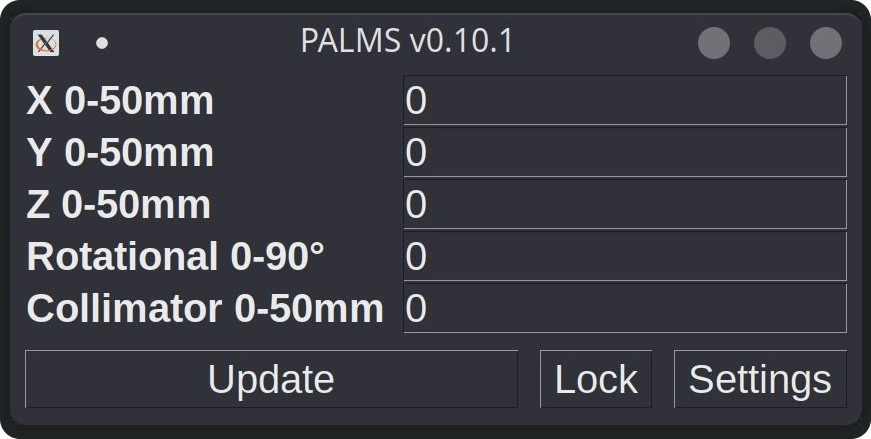
\includegraphics[scale=0.7]{palms-gui}
      \caption{PALMS graphical user interface}
    \end{figure}

  \end{block}

  \begin{block}{User Experience}

    PALMS is designed to be used with minimal engagement from the operator.
    It provides a simple workflow that streamlines data acquisition with LIBS.

    \heading{Features}
    \begin{itemize}
      \item When used in conjunction with a robotized multi-axial optomechanical positioning system, 
      PALMS allows the operator to update the 
      desired planar position (XY), 
      3rd axis distance (Z), 
      angular tilt between alternate optics components (A), 
      and alternate optic distance (B).
      \item PALMS also features a lock functionality that lets the operator lock all of the axes for as long as desired for up to 60 seconds. 
      This enables sample switching 
      and movements in close proximity to the positioning system without risking an unintentional displacement of the sample.

    \end{itemize}

    \heading{See It in Action}

    Scan the QR code below to watch a demonstration.

    \begin{figure}
      \centering
      
\includegraphics[scale=0.035]{demo-qr-link}
    \end{figure}

  \end{block}

\end{column}

\separatorcolumn

\begin{column}{\colwidth}

  \begin{block}{Remote Operation}

    Because the PALMS client and server only need to have a network connection to communicate, 
    the operator can remotely control the robotized positioning system and monitor it via networked cameras.
      
    \begin{itemize}
      \item PALMS allows remote operation under conditions that are not ideal for in person operation, 
      such as a lack of space in the LIBS enclosure, 
      an inability to wear protective gear, 
      telework, 
      and safety concerns if working with hazardous samples.

      \item With remote desktop software, PALMS is globally accessible over the internet.
      \item Educators can let students who are present in person or virtually observe the operation of a LIBS instrument.
    \end{itemize}

    \begin{figure}
      \centering
      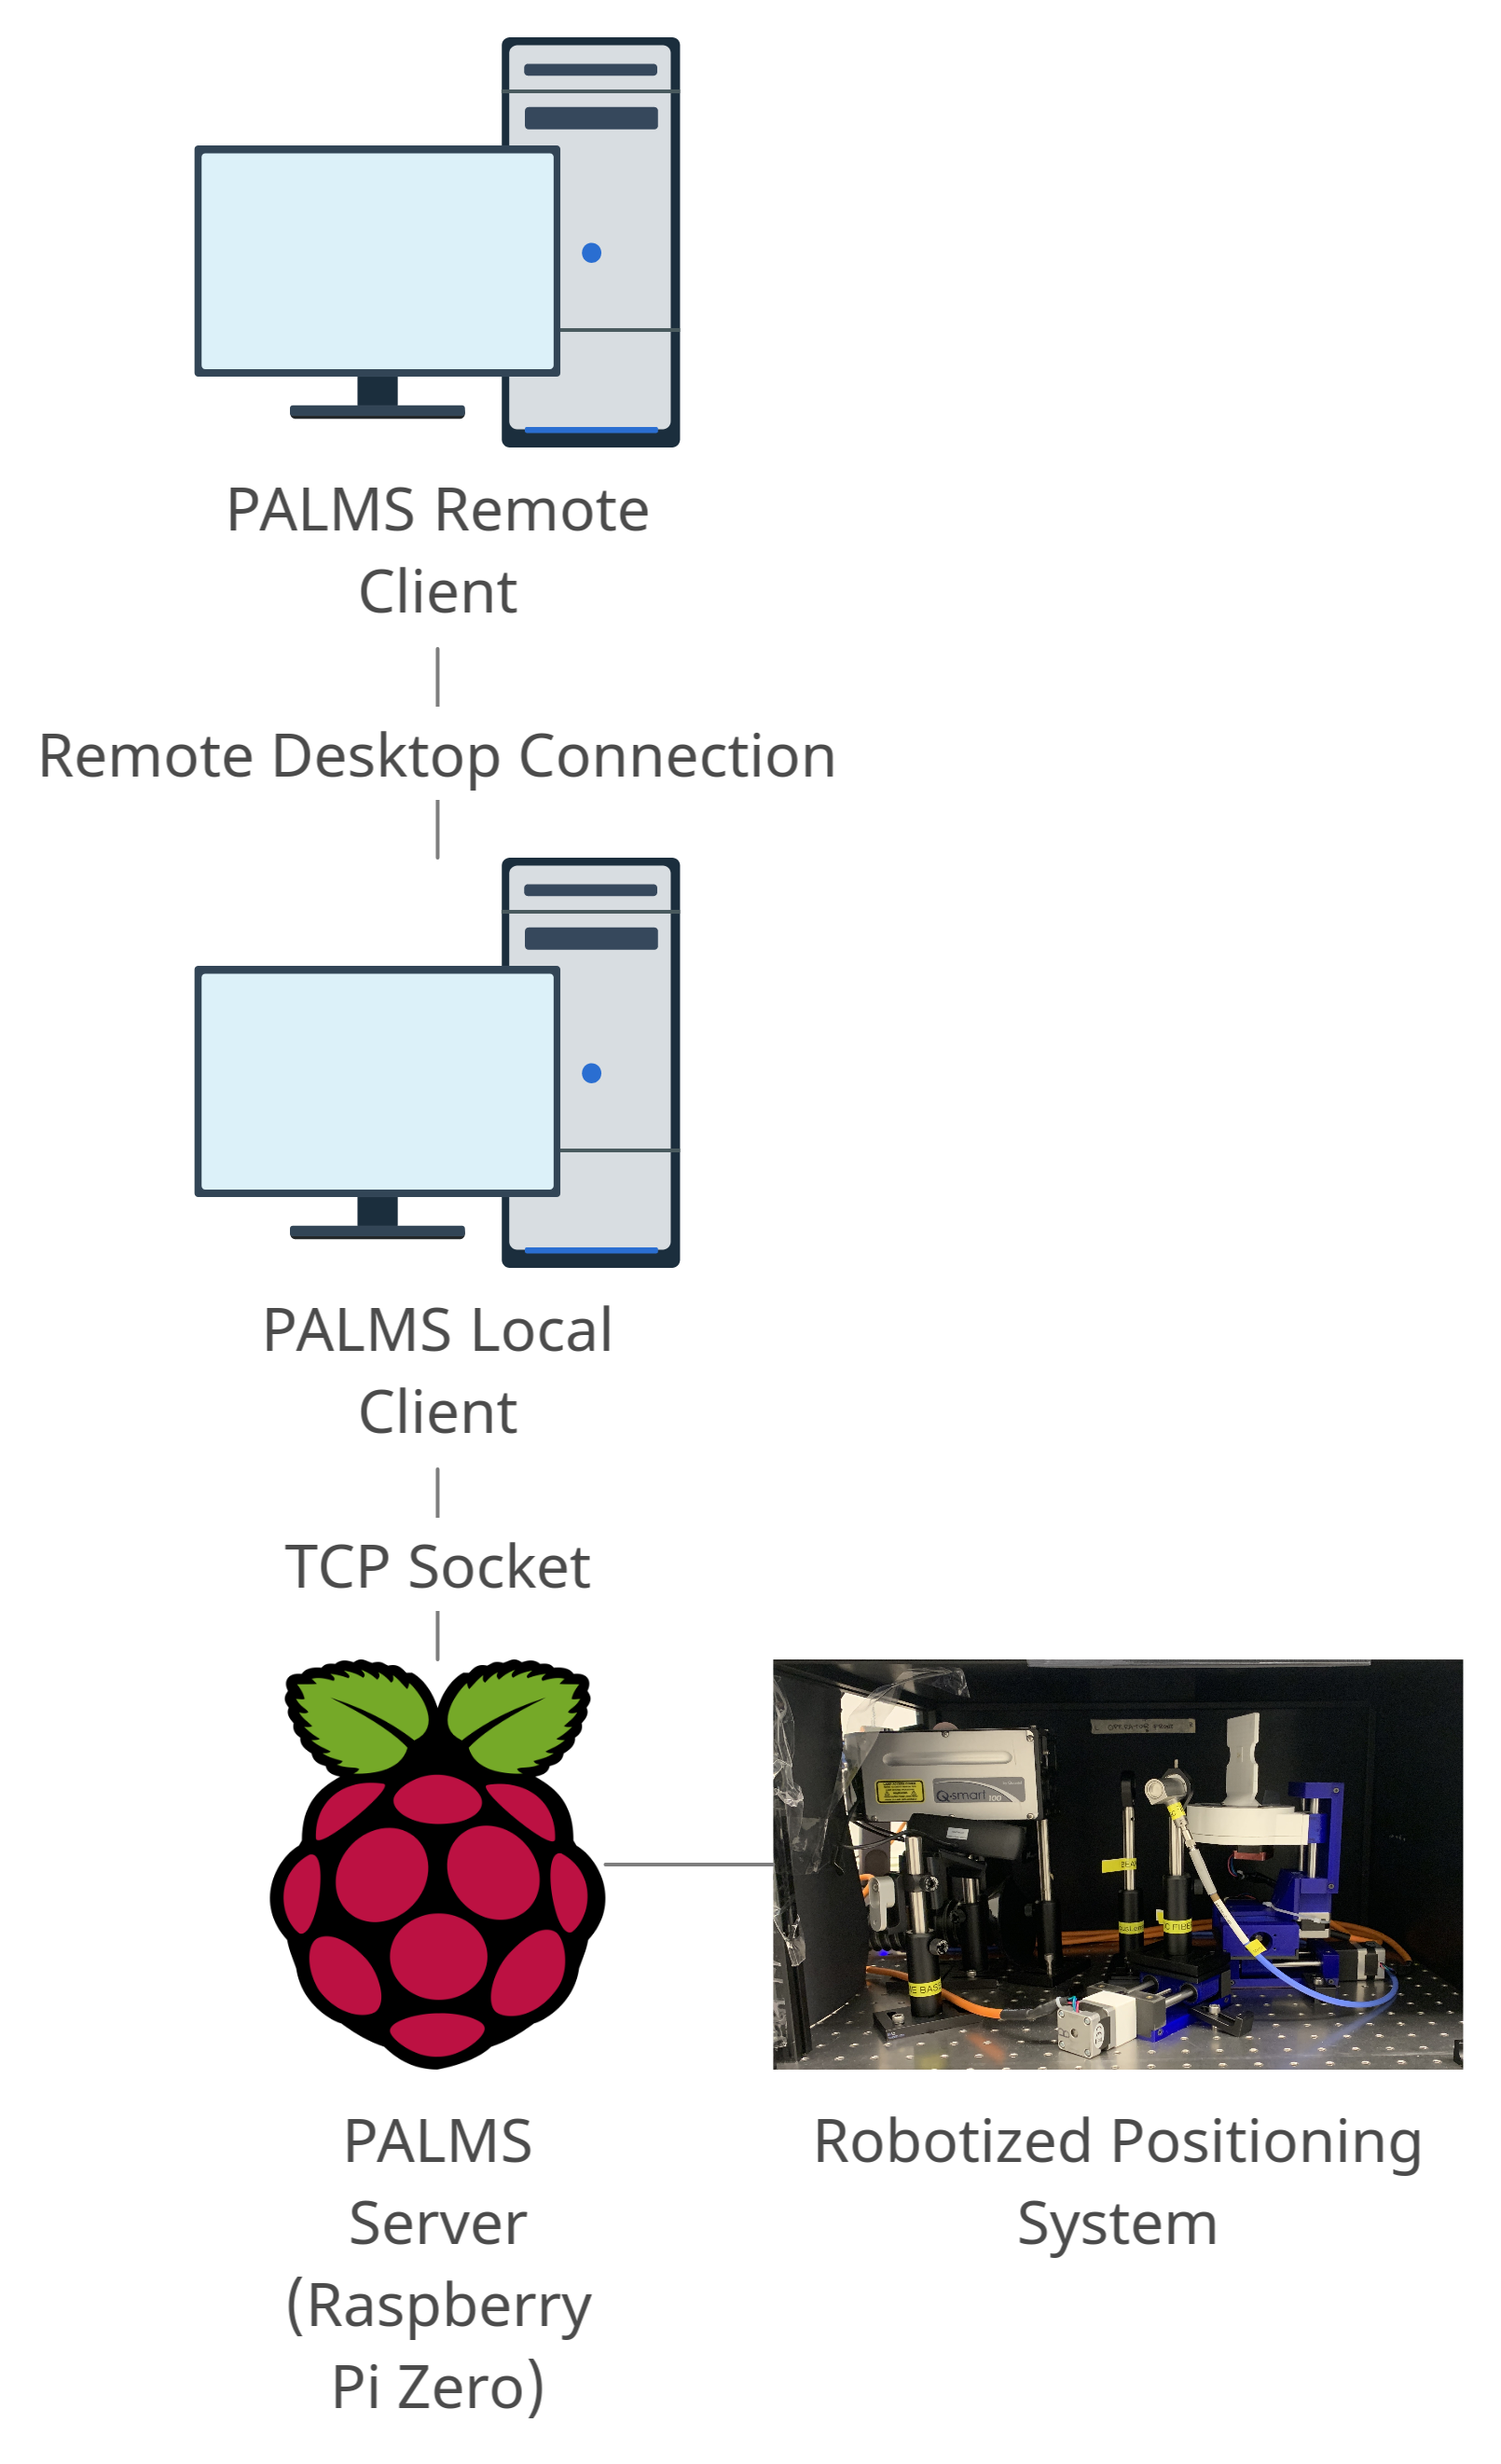
\includegraphics[scale=0.32]{palms-diagram}
      \caption{PALMS component diagram}
    \end{figure}

  \end{block}
  
\end{column}

\separatorcolumn

\begin{column}{\colwidth}

  \begin{block}{Results}

    When PALMS was introduced into the research workflow in our lab, there was an immediate, clearly noticeable benefit.
    With only a few minutes of training, researchers were acquiring data with the LIBS instrument much more 
    effectively, efficiently, and reproducibly than before.
    
    Because the operators could record the exact position of the sample, they could easily and quickly reproduce their results.
    Additionally, they could rapidly analyze a large number of dimensionally similar samples while reducing experimental error.

    When collaborating, researchers also found that the ability to remotely adjust the sample position 
    and the capability to remotely observe via networked cameras invaluable.
    Furthermore, several team members were able to telework without detriment to the quality of their LIBS data.

  \end{block}

  \begin{block}{Conclusion}

    PALMS shows that successful scientific research requires well-built scientific software.
    \textbf{During testing, researchers using PALMS reported that it was 
    easily usable, 
    reliable, 
    and provided a much needed optimization for LIBS.
    Without the aforementioned qualities guaranteed by PALMS, 
    much of the research conducted in our lab would have been much more difficult and arduous to complete.}
    The PALMS project allows robotized optomechanical systems to deliver their full potential.

  \end{block}

  \begin{block}{References}

    \nocite{*}
    \footnotesize{\bibliographystyle{plain}\bibliography{scix-poster}}

  \end{block}

\end{column}

\separatorcolumn
\end{columns}
\end{frame}

\end{document}
